\section{Prior Work and Motivation}

\begin{frame}{What is an Impact Model?}
    \begin{itemize}
        \item Predicts behavior of an object after contact with another object (e.g. Cassie's Foot with Ground) \\
    \end{itemize}    
    \newline
    \tikzstyle{startstop} = [rectangle, rounded corners, minimum width=3.5cm, minimum height=1.75cm, text centered, text width = 4cm, draw=black]
    \tikzstyle{arrow} = [ultra thick,->,>=stealth]
    \begin{tikzpicture}[node distance=2cm]
    
        \node (in) [startstop, label=above:{\textbf{Input}}, xshift = 2cm, yshift = 10cm] { $v^-$ \\(pre-impact velocity, position, and orientation) \\ };
        \node (out) [startstop, label=above:{\textbf{Output}}, xshift = 8cm, yshift = 10 cm] {$v^+$ \\(post-impact velocity, position, and orientation)};
        \node(props)  [startstop, label=above:{\textbf{System Properties}}, width=6cm, xshift = 5cm, yshift = 7.5cm] { $\mu$ (frictional coefficient)\\ $\epsilon$ (coefficient of restitution)};
        \draw [arrow] (in) -- (out) node[midway,above] {\textit{Model}};

    \end{tikzpicture}

\end{frame}


\begin{frame}
\frametitle{Prior Work (Dr.\ Nima Fazeli)}

\begin{itemize}
    \item Paper's Goal - Compare and evaluate impact models \\
    \begin{itemize}
    \item Tuned system properties to enhance the performance of the models 
    \end{itemize}
    \item Data - Planar impacts from 3D printed ellipses \\
\end{itemize}

\begin{figure}[h!]
    \centering
    \begin{subfigure}[b]{0.5\linewidth}
        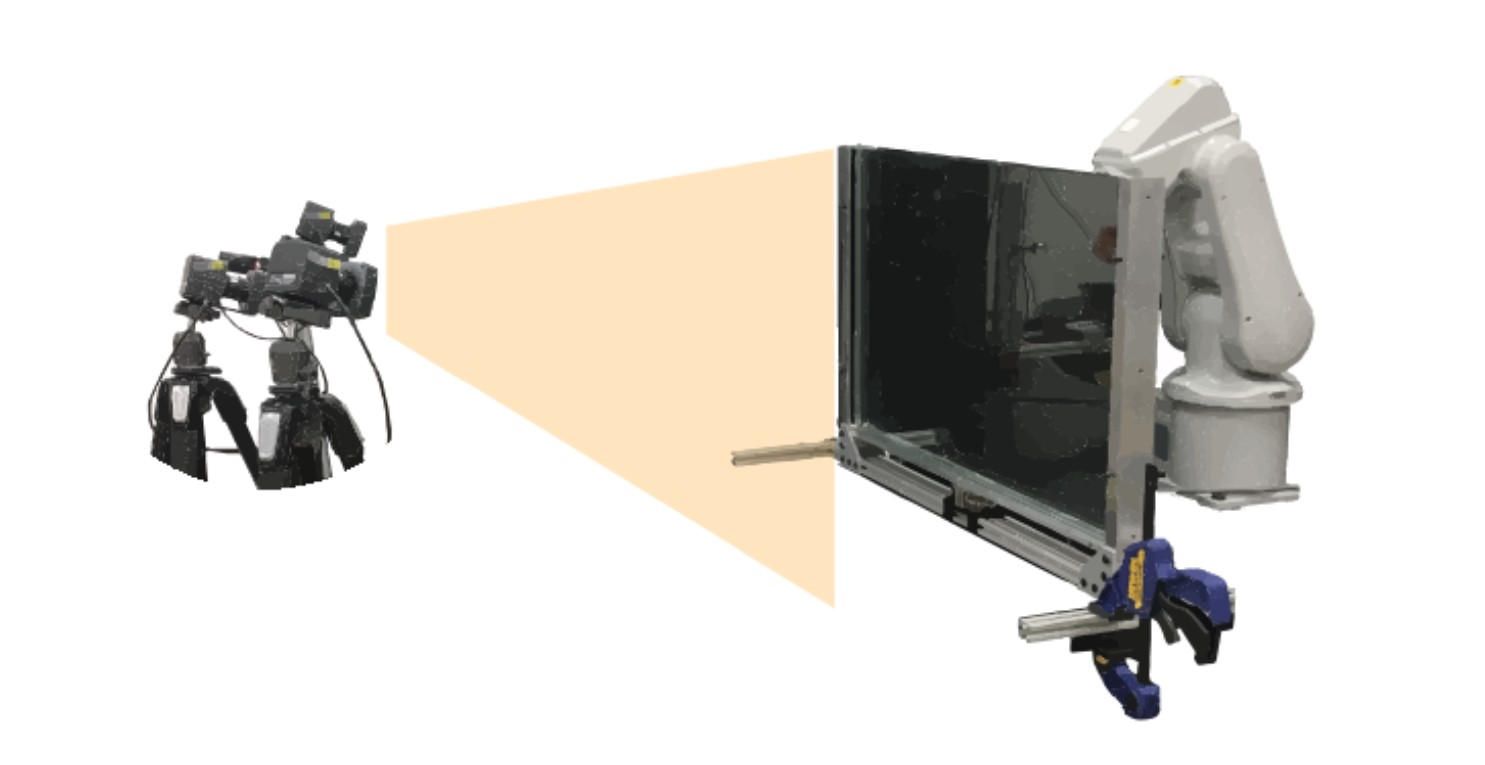
\includegraphics[scale=0.4]{figures/nimaFigSetup.jpg}
        \caption{Experimental Setup\cite{nima1}}
        \label{fig:cIRB}
    \end{subfigure}
    \quad
    \begin{subfigure}[b]{0.4\linewidth}
       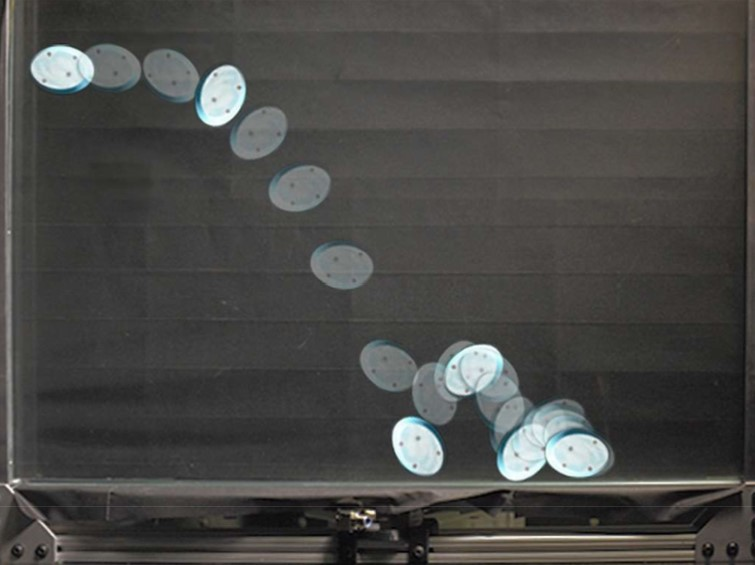
\includegraphics[scale=0.5]{figures/nimaFigDrop.jpg}
        \caption{Dropping Ellipse\cite{nima1}\cite{nima2}}
        \label{fig:nimaDrop}
    \end{subfigure}
\end{figure}

\end{frame}

\setlength{\belowcaptionskip}{-10pt}
\begin{frame}{Prior Work  (Dr.\ Nima Fazeli)}
    Key Takeaways \\
    \begin{itemize}
        \item None of the predictive models are very good
        \item Even post-hoc models like IRB have significant error
    \end{itemize}
 \begin{figure}
        \centering
        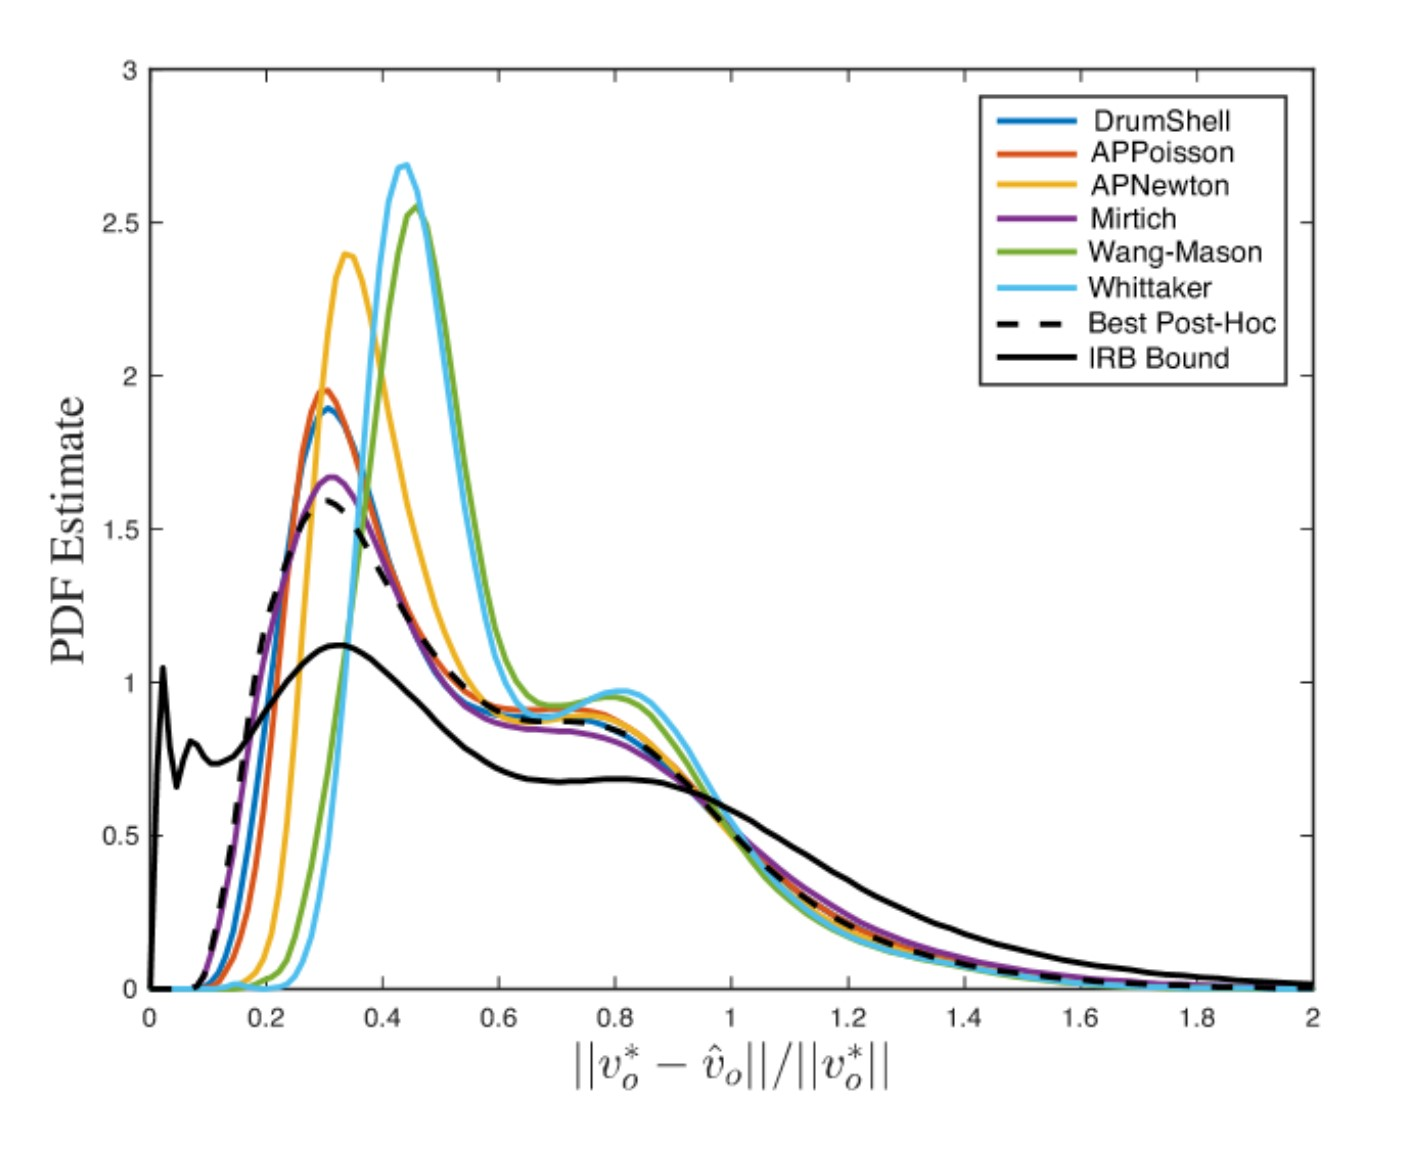
\includegraphics[scale=0.35]{figures/nimaFigModels.jpg}
        \caption{frequency of Errors Across Different impact Models\cite{nima2}}
        \label{fig:nimaModels}
\end{figure}
\end{frame}

\subsection{Research Goals}
\begin{frame}{Research Goals}
\begin{itemize}
    \item Understand a few impact models
    \item Experiment with interesting data sets and compare to work done by Dr. Fazeli
    \item Look for issues and shortcomings from models
    \item Test different ways to improve models
\end{itemize}
\end{frame}   


